\documentclass{article}
\usepackage[utf8]{inputenc}
\usepackage[T1]{fontenc}
\usepackage{graphicx}
\usepackage{hyperref}
\usepackage{geometry}
\geometry{margin=1in}

\title{T H O T H R}
\date{Encyclopaedia Britannica (1771)}

\begin{document}
\maketitle

\section*{Historical source}
\textbf{Entry ID:} \texttt{entry-t-h-o-t-h-r-604} \\
\textbf{Volume ID:} 193819047 \\
\textbf{Character Count:} 1200

\subsection*{Extracted Text}
Thoos. attended, walking as mourners. The queen and princesses also assisted at the ceremony of people including the public bodies, mountains and ascidental, amoured to many thousands. An interesting part of the ceremony was the performance of a woman written by the sculptor’s initiale and the friend of Manchester.

Thowments was rather above the middle height, firmly build, with broad shoulders. The owner of his face was rather square. His general expression was calm and thoughtful, and very pleasing. His eyes were light and penetrating; his mouth wide and usually enjoyable. He wore his hair, and had grown nearly white in large masses divided over his fine than forefoot, and killing on each side, something like a lion’s mane, nearly to his shoulders.

Thornflies we all always ask me walk van Cuavaa and Flacman as one of the great representatives of Sculpture. The former, his sliders were almost the first to break through the intensive routine of the world mixed Italian and French art which had descended from Bernent and his school. Thornalizes nobly asked in advancing this revoltion, and with them assisted in establishing the practice of sculpture upon true principles. (a. w.-r.).

\subsection*{Matched Wikipedia Article}
\textbf{Title:} Neomirandea \\
\textbf{Page ID:} 23667568 \\
\textbf{Revision ID:} 1086015190 \\
\textbf{URL:} \url{https://en.wikipedia.org/wiki/Neomirandea}


\section*{Source record}
\begin{itemize}
\item \textbf{Dataset:} \texttt{NationalLibraryOfScotland/encyclopaedia\_britannica\_illustrated}
\item \textbf{Dataset Revision:} \texttt{309f765b1ecc83e0a7f7762e44b4a927a7555443}
\item \textbf{Page ID:} \texttt{britannica:309f765b1ecc83e0a7f7762e44b4a927a7555443:train:604} \\
  \textbf{Filename:} \texttt{page-0604-c50a825dd732.jpg} \\
  \textbf{Row Index:} 604 \\
  \textbf{SHA256:} \texttt{c50a825dd732a96e...}
\end{itemize}

\begin{figure}[h]
\centering
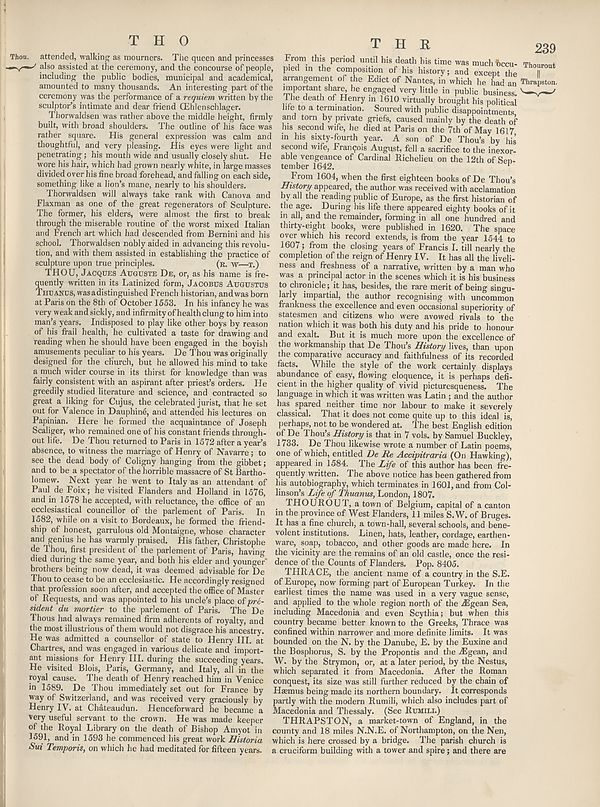
\includegraphics[width=0.85\textwidth]{../scans/page-0604-c50a825dd732.jpg}
\caption*{Source scan: \texttt{page-0604-c50a825dd732.jpg}}
\end{figure}

\end{document}
